\section{Introduction}

As the availability of genetic data has increased,
so has our ability to infer evolutionary processes at finer scales.
An essential tool for evolutionary inference has been simulations,
and many flexible and efficient evolutionary simulators have been developed over the past decade.
Until recently, little had been done to integrate different tools and to ensure compatibility of inferred models across studies.

A unifying thread that has emerged is the use of tree sequence data structure.
The tree sequence provides a way of concisely representing correlated genealogies along chromosomes.
Further, it 

\section{Parallelizing forward-in-time simulations}

A major problem in simulation-based inference is the computational cost of simulations.
In many cases, it is possible to minimize the time cost of simulations by running them in parallel,
that is to divide up the simulation over many processes that can be executed concurrently over many CPUs (or cores).
It is not always that it is clear how to divide a simulation into sub-tasks.

In the case of evolutionary simulations, a natural way to break up a big simulation might be population splits.
After a population splits into two (or more) subpopulations, their histories become independent (assuming no migration).
Therefore, it is possible to parallelize a multi-population simulation by dividing the simulation over population splits.
The history of populations A, B and C (shown in \lcref{fig:pop_hist}) can be parallelized:
any two branches stemming from the same node are independent.

\begin{figure}[htp]
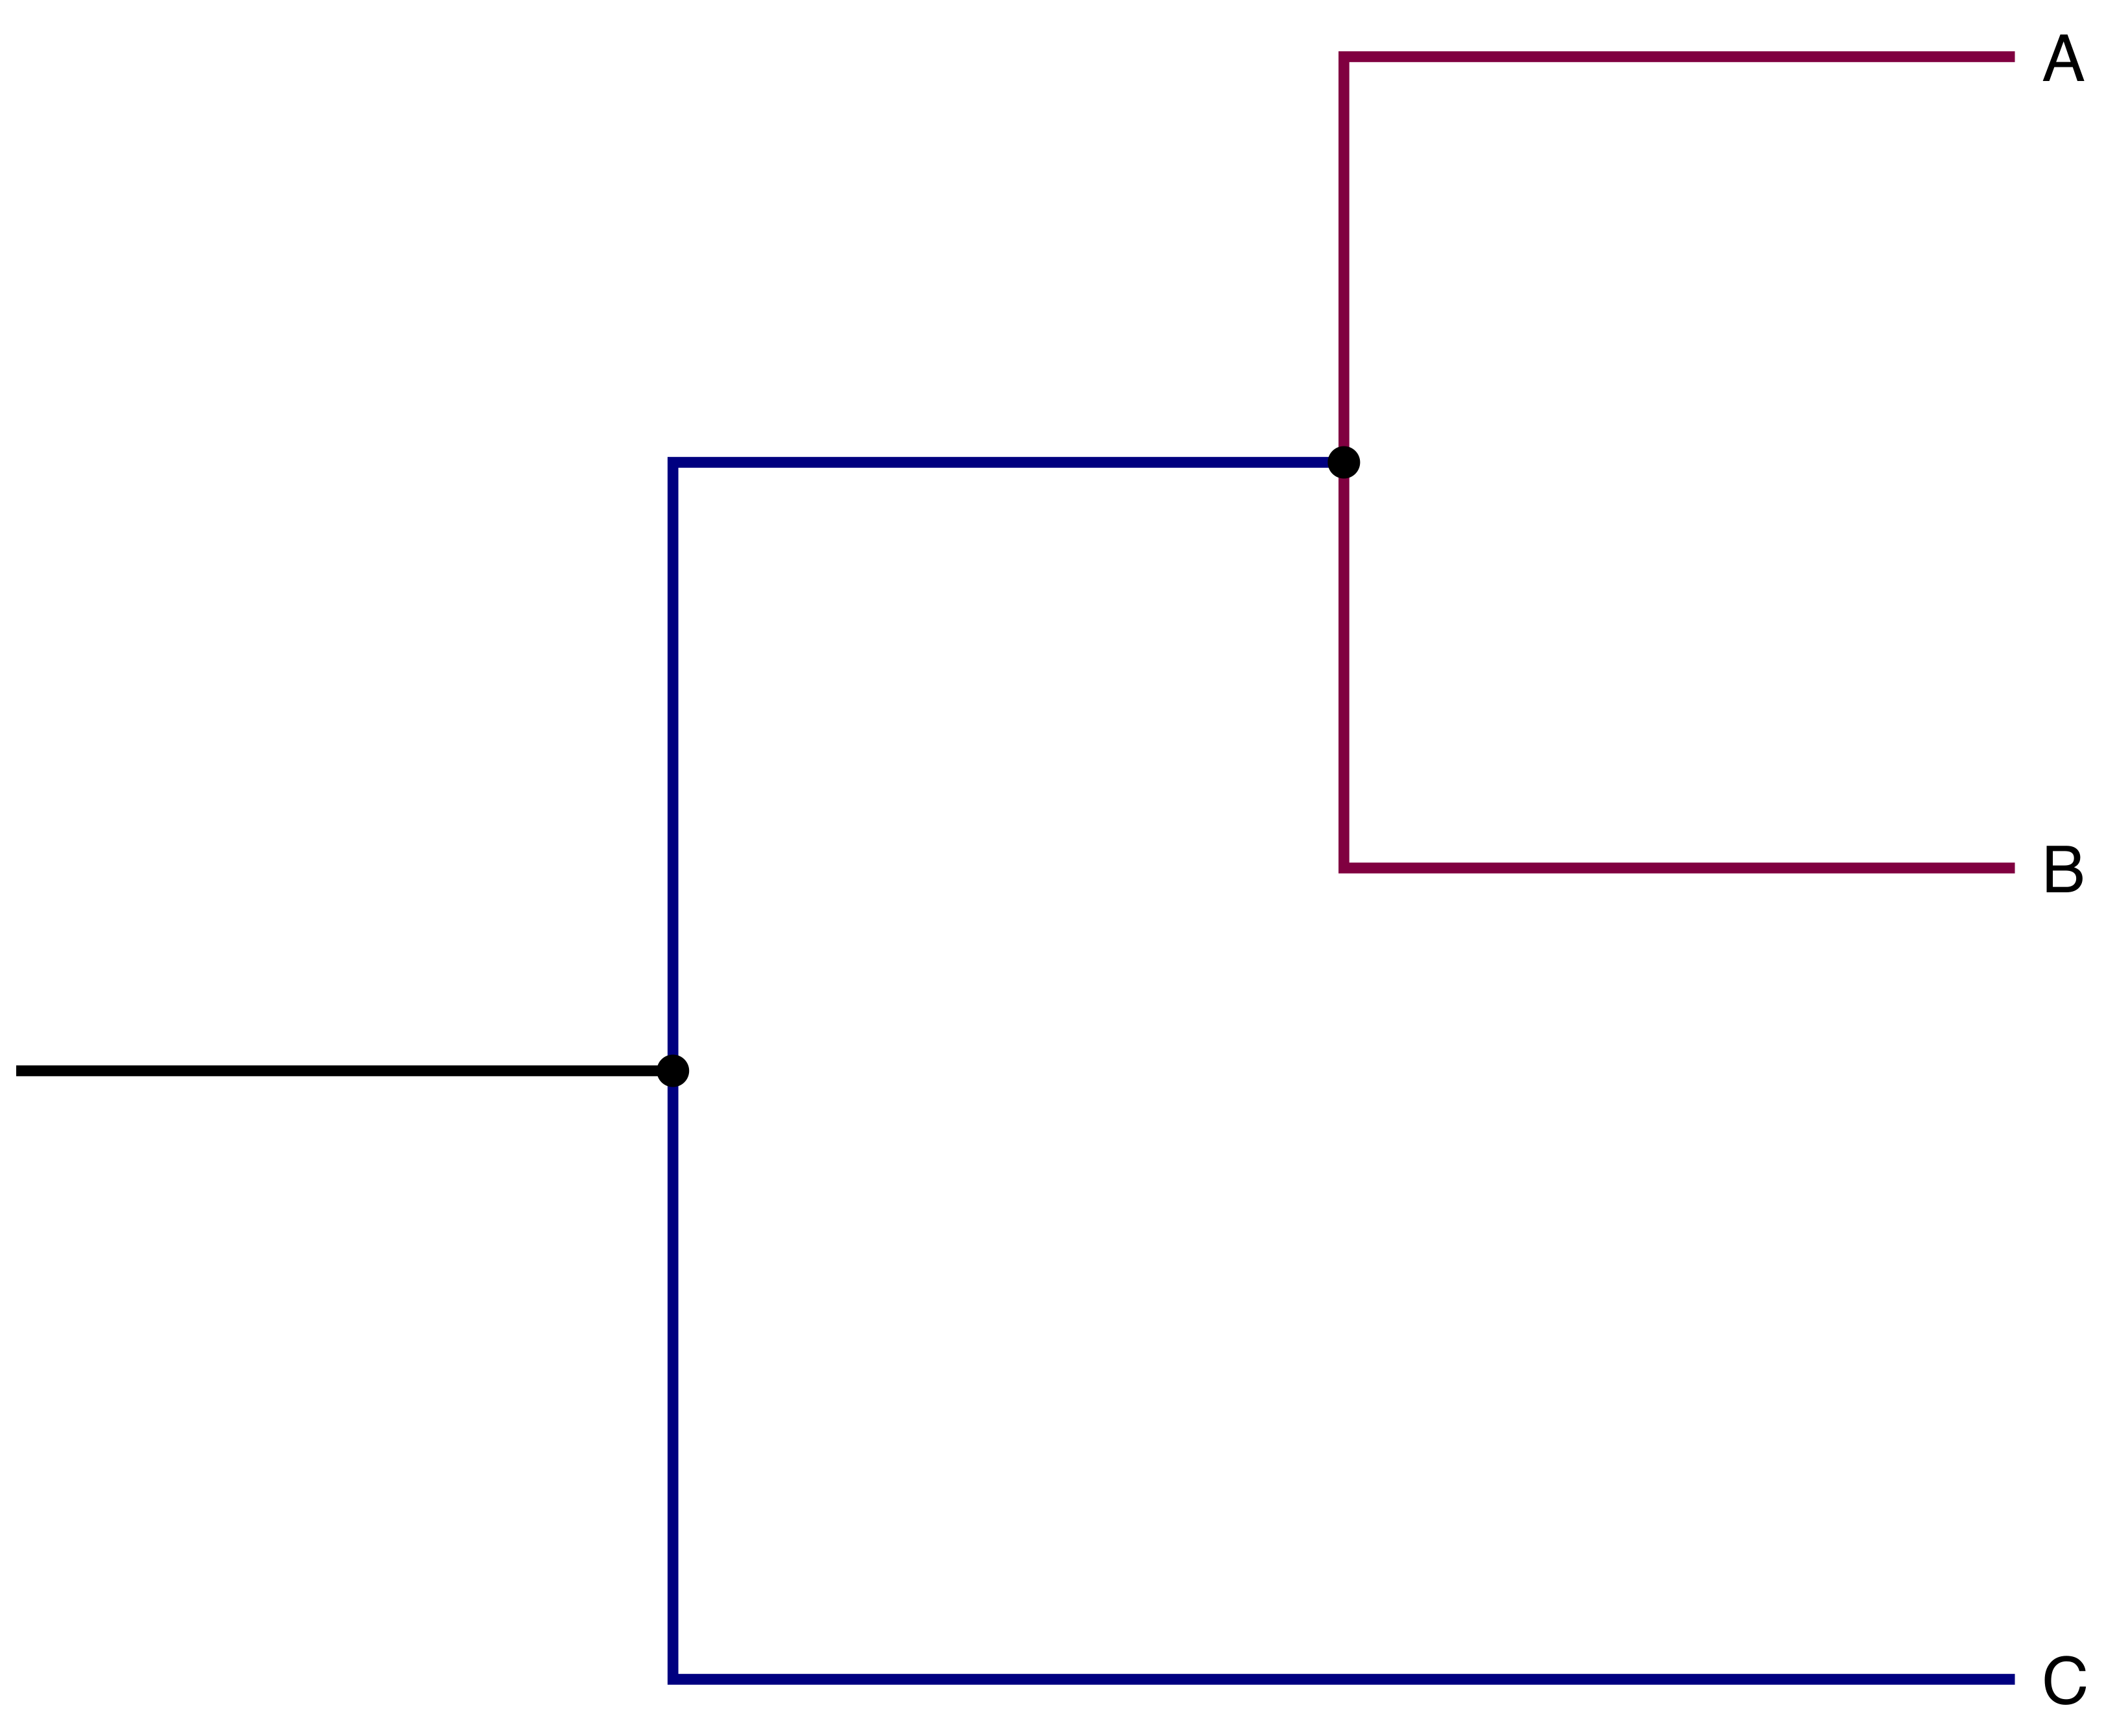
\includegraphics[width=0.5\linewidth]{{figures/phylo.png}}
\centering
\caption[Example of a population history]{
The relationships between populations A, B and C are depicted.
Note how branches of the same color can be simulated in parallel if there is no migration.
}
\label{fig:pop_hist}
\end{figure}


